\documentclass[twocolumn]{article}

\usepackage{tikz}
\usetikzlibrary{arrows}

\begin{document}

%\chapter{Programming Languages}
%
%\section{Textual Languages}
%
%\section{Visual Languages}
%
%\subsection{Why Visual Languages}
%
%\subsection{Domain Specific}
%
%
%\section{Existing Visual Languages}
%
%\subsection{The Bad}
%\subsection{General Visual Languages}
%
%
%\section{Area of improvement}
%\subsection{lack of expression}
%
%\subsection{higher order concepts} 
%
%\subsection{higher order syntax}
%
%\subsection{higher order semantics} 
%
%\chapter{Data Manipulation Language Design}

To start with, a visual language for data manipulation should most likely be
similar to other dataflow languages.  It should be able to handle the idea of
messaging and therefore be multithreaded.

I immediately go to functional programming for a variety of reasons, many of 
which are.


% these two should merge into something....probably nameless
%\section{Use Cases}
%\section{Functional}

\section{Basic Language}


\subsection*{Nodes}


\begin{tikzpicture}
    \draw [fill] (0.5, 0.5) circle [radius=0.5];
    \node [below] at (0.5, 0) { value };

    \draw [thick] (2.5, 0.5) circle [radius=0.5]; 
    \node [below] at (2.5, 0) { type };

    \draw [fill] (4.5, 0.5) circle [radius=0.5];  
    \draw[white,ultra thick] (4.5, 0.5) circle [radius=0.4]; 
    \node [align=center,below] at (4.5, 0)%
       {bound type};
\end{tikzpicture}

\subsection*{Arrows}

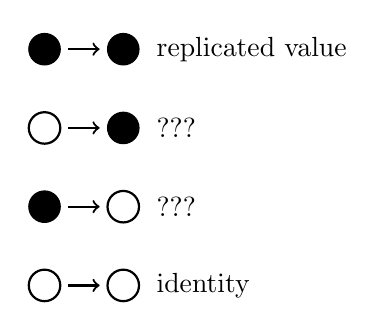
\begin{tikzpicture}
    \draw [fill] (0,0) circle [radius=0.2];
    \draw [fill] (1,0) circle [radius=0.2];
    \draw [->,thick] (0.3,0) -- (0.7,0);
    \node [right] at (1.3,0)%
        {replicated value};

    \draw [thick] (0,-1) circle [radius=0.2];
    \draw [fill] (1,-1) circle [radius=0.2];
    \draw [->,thick] (0.3,-1) -- (0.7,-1);
    \node [right] at (1.3,-1)%
        {???};

    \draw [fill] (0,-2) circle [radius=0.2];
    \draw [thick] (1,-2) circle [radius=0.2];
    \draw [->,thick] (0.3,-2) -- (0.7,-2);
    \node [right] at (1.3,-2)%
        {???};

    \draw [thick] (0,-3) circle [radius=0.2];
    \draw [thick] (1,-3) circle [radius=0.2];
    \draw [->,thick] (0.3,-3) -- (0.7,-3);
    \node [right] at (1.3,-3)%
        {identity};
\end{tikzpicture}

\subsubsection*{Functions}


\subsubsection*{Infix}
\subsubsection*{Joins}
\subsubsection*{Recursion}

\subsection{Contexts}
\subsubsection*{Widgets}
\subsection{Externs}
\subsection{Sugars}
\subsubsection*{}
\subsubsection*{Infix}
\subsubsection*{Recursion}

\section{Higher Order Types}

\end{document}
